\documentclass[conference]{IEEEtran}
\usepackage[utf8]{inputenc}
\usepackage[spanish]{babel}
\usepackage{amsmath,amssymb,amsfonts}
\usepackage{graphicx}
\usepackage{booktabs}
\usepackage{cite}
\usepackage{url}

\begin{document}

\title{Estudio Comparativo de Clasificadores Supervisados para la Predicción de Suscripción a Depósitos Bancarios: Naive Bayes, SVM y Perceptrón Multicapa}

\author{\IEEEauthorblockN{Luis Fernando Cruz Villegas}
\IEEEauthorblockA{\textit{Licenciatura en Ingeniería en Computación} \\
\textit{Centro Universitario UAEM Texcoco -- Universidad Autónoma del Estado de México}\\
Texcoco, Estado de México, México \\
lcruzv@alumno.uaemex.mx}}

\maketitle

\begin{abstract}
Las campañas de marketing directo en el sector financiero enfrentan el reto de optimizar los recursos de contacto telefónico frente a tasas de conversión históricamente bajas. Este trabajo presenta un estudio experimental reproducible que compara tres paradigmas de aprendizaje supervisado ---Clasificador Bayesiano Ingenuo Gaussiano (Gaussian Naive Bayes), Máquinas de Soporte Vectorial (SVM) con núcleos lineal y de base radial (RBF), y un Perceptrón Multicapa (MLP)--- frente a una línea base de Regresión Logística, utilizando el conjunto de datos público \textit{Bank Marketing} de UCI (45,211 registros). Para evitar fuga de datos, se excluyó la duración de llamada y se aplicó un flujo de preprocesamiento ajustado exclusivamente sobre la partición de entrenamiento (70\%), evaluando mediante validación cruzada estratificada de 5 pliegues y un conjunto de prueba independiente (15\%). Los resultados se analizan bajo métricas sensibles al desbalance de clases (F1-Score, ROC-AUC y PR-AUC). Se demuestra que los modelos no lineales (SVM-RBF y MLP) capturan interacciones complejas entre variables socioeconómicas y el historial de contacto, superando significativamente los supuestos de independencia condicional de Naive Bayes.
\end{abstract}

\begin{IEEEkeywords}
Aprendizaje supervisado, clasificación desbalanceada, máquinas de soporte vectorial, naive bayes, perceptrón multicapa, marketing bancario.
\end{IEEEkeywords}

\section{Introducción}
El marketing directo mediante centros de contacto telefónico constituye una estrategia central para que las instituciones bancarias promuevan productos financieros como los depósitos a plazo fijo. Sin embargo, las campañas masivas no segmentadas generan altos costos operativos, fatiga en el cliente y tasas de rechazo superiores al 88\% \cite{moro2014}. En este contexto, la Ciencia de Datos permite construir modelos predictivos que estiman la propensión de cada cliente a contratar un producto antes de realizar la llamada.

El problema presenta desafíos técnicos relevantes: coexisten variables numéricas con distribuciones altamente sesgadas, atributos categóricos nominales, y un pronunciado desbalance de clases donde la clase positiva representa apenas una fracción minoritaria de la población. Bajo estas condiciones, métricas tradicionales como la exactitud global (\textit{accuracy}) resultan engañosas, pues un clasificador trivial que prediga siempre la clase negativa alcanzaría cerca del 88.3\% de acierto sin aportar valor comercial.

La contribución de este trabajo consiste en diseñar, implementar y evaluar bajo un protocolo experimental libre de fuga de datos (\textit{data leakage}) tres familias de algoritmos de clasificación supervisada: un modelo probabilístico generativo (Naive Bayes), un clasificador de margen máximo basado en teoría del aprendizaje estadístico (SVM) y una arquitectura conexionista profunda (Perceptrón Multicapa), contrastándolos contra una Regresión Logística regularizada. Todo el flujo se implementa con semillas fijas para garantizar plena reproducibilidad computacional.

\section{Trabajo Relacionado}
La aplicación de técnicas de minería de datos y aprendizaje automático al conjunto \textit{Bank Marketing} ha sido ampliamente estudiada en la literatura. Moro et al. \cite{moro2014} introdujeron originalmente este conjunto de datos recopilado de una institución bancaria portuguesa, evaluando regresión logística, árboles de decisión, redes neuronales y máquinas de soporte vectorial, concluyendo que las redes neuronales alcanzaban el mayor área bajo la curva ROC al incorporar indicadores macroeconómicos.

Posteriormente, Elsalamony \cite{elsalamony2014} comparó perceptrones multicapa, árboles C5.0 y regresión logística sobre campañas bancarias, destacando la sensibilidad de los modelos ante la codificación de variables categóricas. En el ámbito del manejo de clases desbalanceadas, Chawla et al. \cite{chawla2002} y Saito y Rehmsmeier \cite{saito2015} demostraron que las curvas Precisión-Recall (PR-AUC) ofrecen una evaluación mucho más informativa que las curvas ROC cuando la prevalencia de la clase positiva es baja.

Respecto a los fundamentos algorítmicos evaluados en este estudio, Cortes y Vapnik \cite{cortes1995} establecieron el marco de las Máquinas de Soporte Vectorial y la proyección a espacios de alta dimensión mediante funciones núcleo (\textit{kernels}), mientras que Zhang \cite{zhang2004} analizó las condiciones de optimalidad del clasificador Naive Bayes a pesar de la violación sistemática de su supuesto de independencia condicional entre atributos. Asimismo, Rumelhart et al. \cite{rumelhart1986} sentaron las bases del entrenamiento de redes multicapa mediante retropropagación del error.

\section{Metodología}

\subsection{Descripción y Análisis Exploratorio de los Datos}
Se empleó el conjunto de datos \textit{Bank Marketing} del repositorio UCI \cite{moro2014}, compuesto por $N = 45,211$ instancias y 16 variables predictoras originales más la etiqueta binaria objetivo $y \in \{\text{no}, \text{yes}\}$. La Fig. \ref{fig:class_dist} evidencia el desbalance de clases: aproximadamente 88.3\% de rechazo frente a 11.7\% de suscripciones exitosas.

\begin{figure}[htbp]
\centering
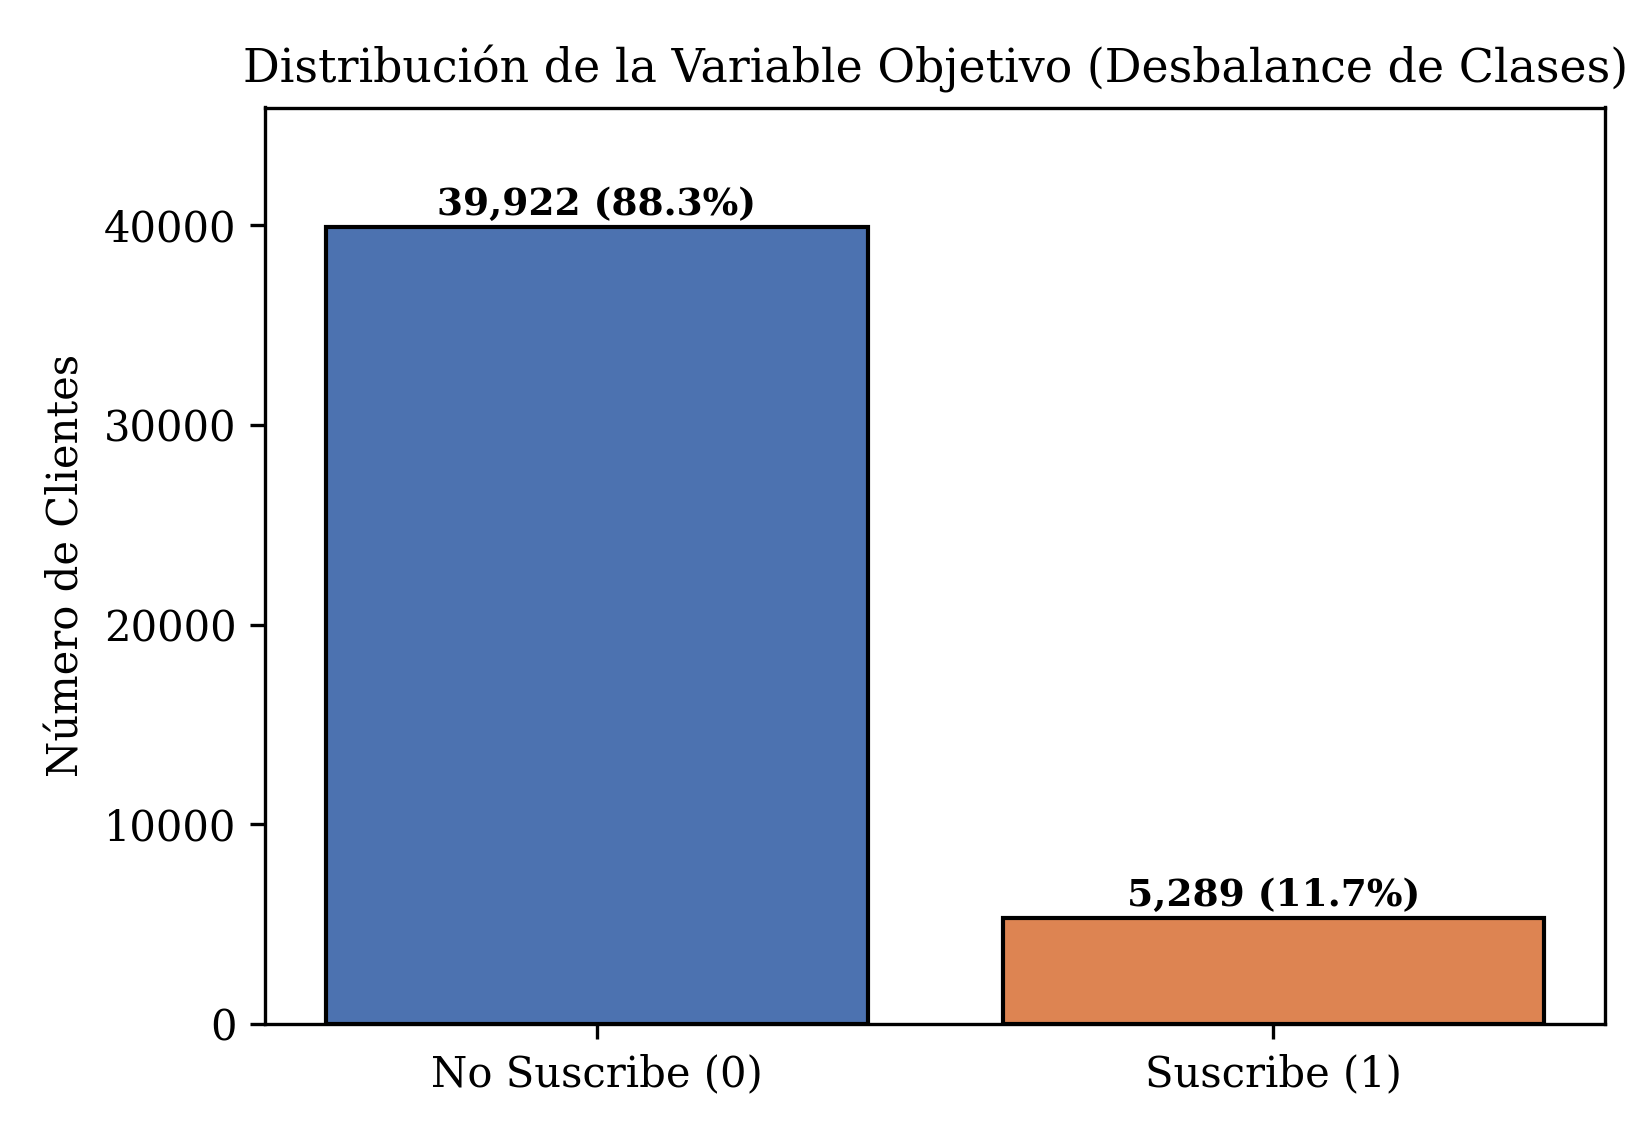
\includegraphics[width=0.88\columnwidth]{figures/fig1_class_distribution.png}
\caption{Distribución de frecuencias y porcentajes de la variable objetivo en el conjunto Bank Marketing.}
\label{fig:class_dist}
\end{figure}

El análisis exploratorio reveló tres hallazgos críticos: (1) existen valores faltantes codificados como categorías desconocidas (\texttt{unknown}) en variables como \texttt{job}, \texttt{education} y \texttt{poutcome}; (2) variables numéricas como \texttt{balance} (saldo promedio anual) y \texttt{campaign} presentan fuerte asimetría positiva y valores atípicos (Fig. \ref{fig:num_dist}); y (3) la matriz de correlación (Fig. \ref{fig:corr}) muestra baja colinealidad lineal entre variables demográficas, pero una relación directa entre \texttt{pdays} (días desde el último contacto) y \texttt{previous}.

\begin{figure}[htbp]
\centering
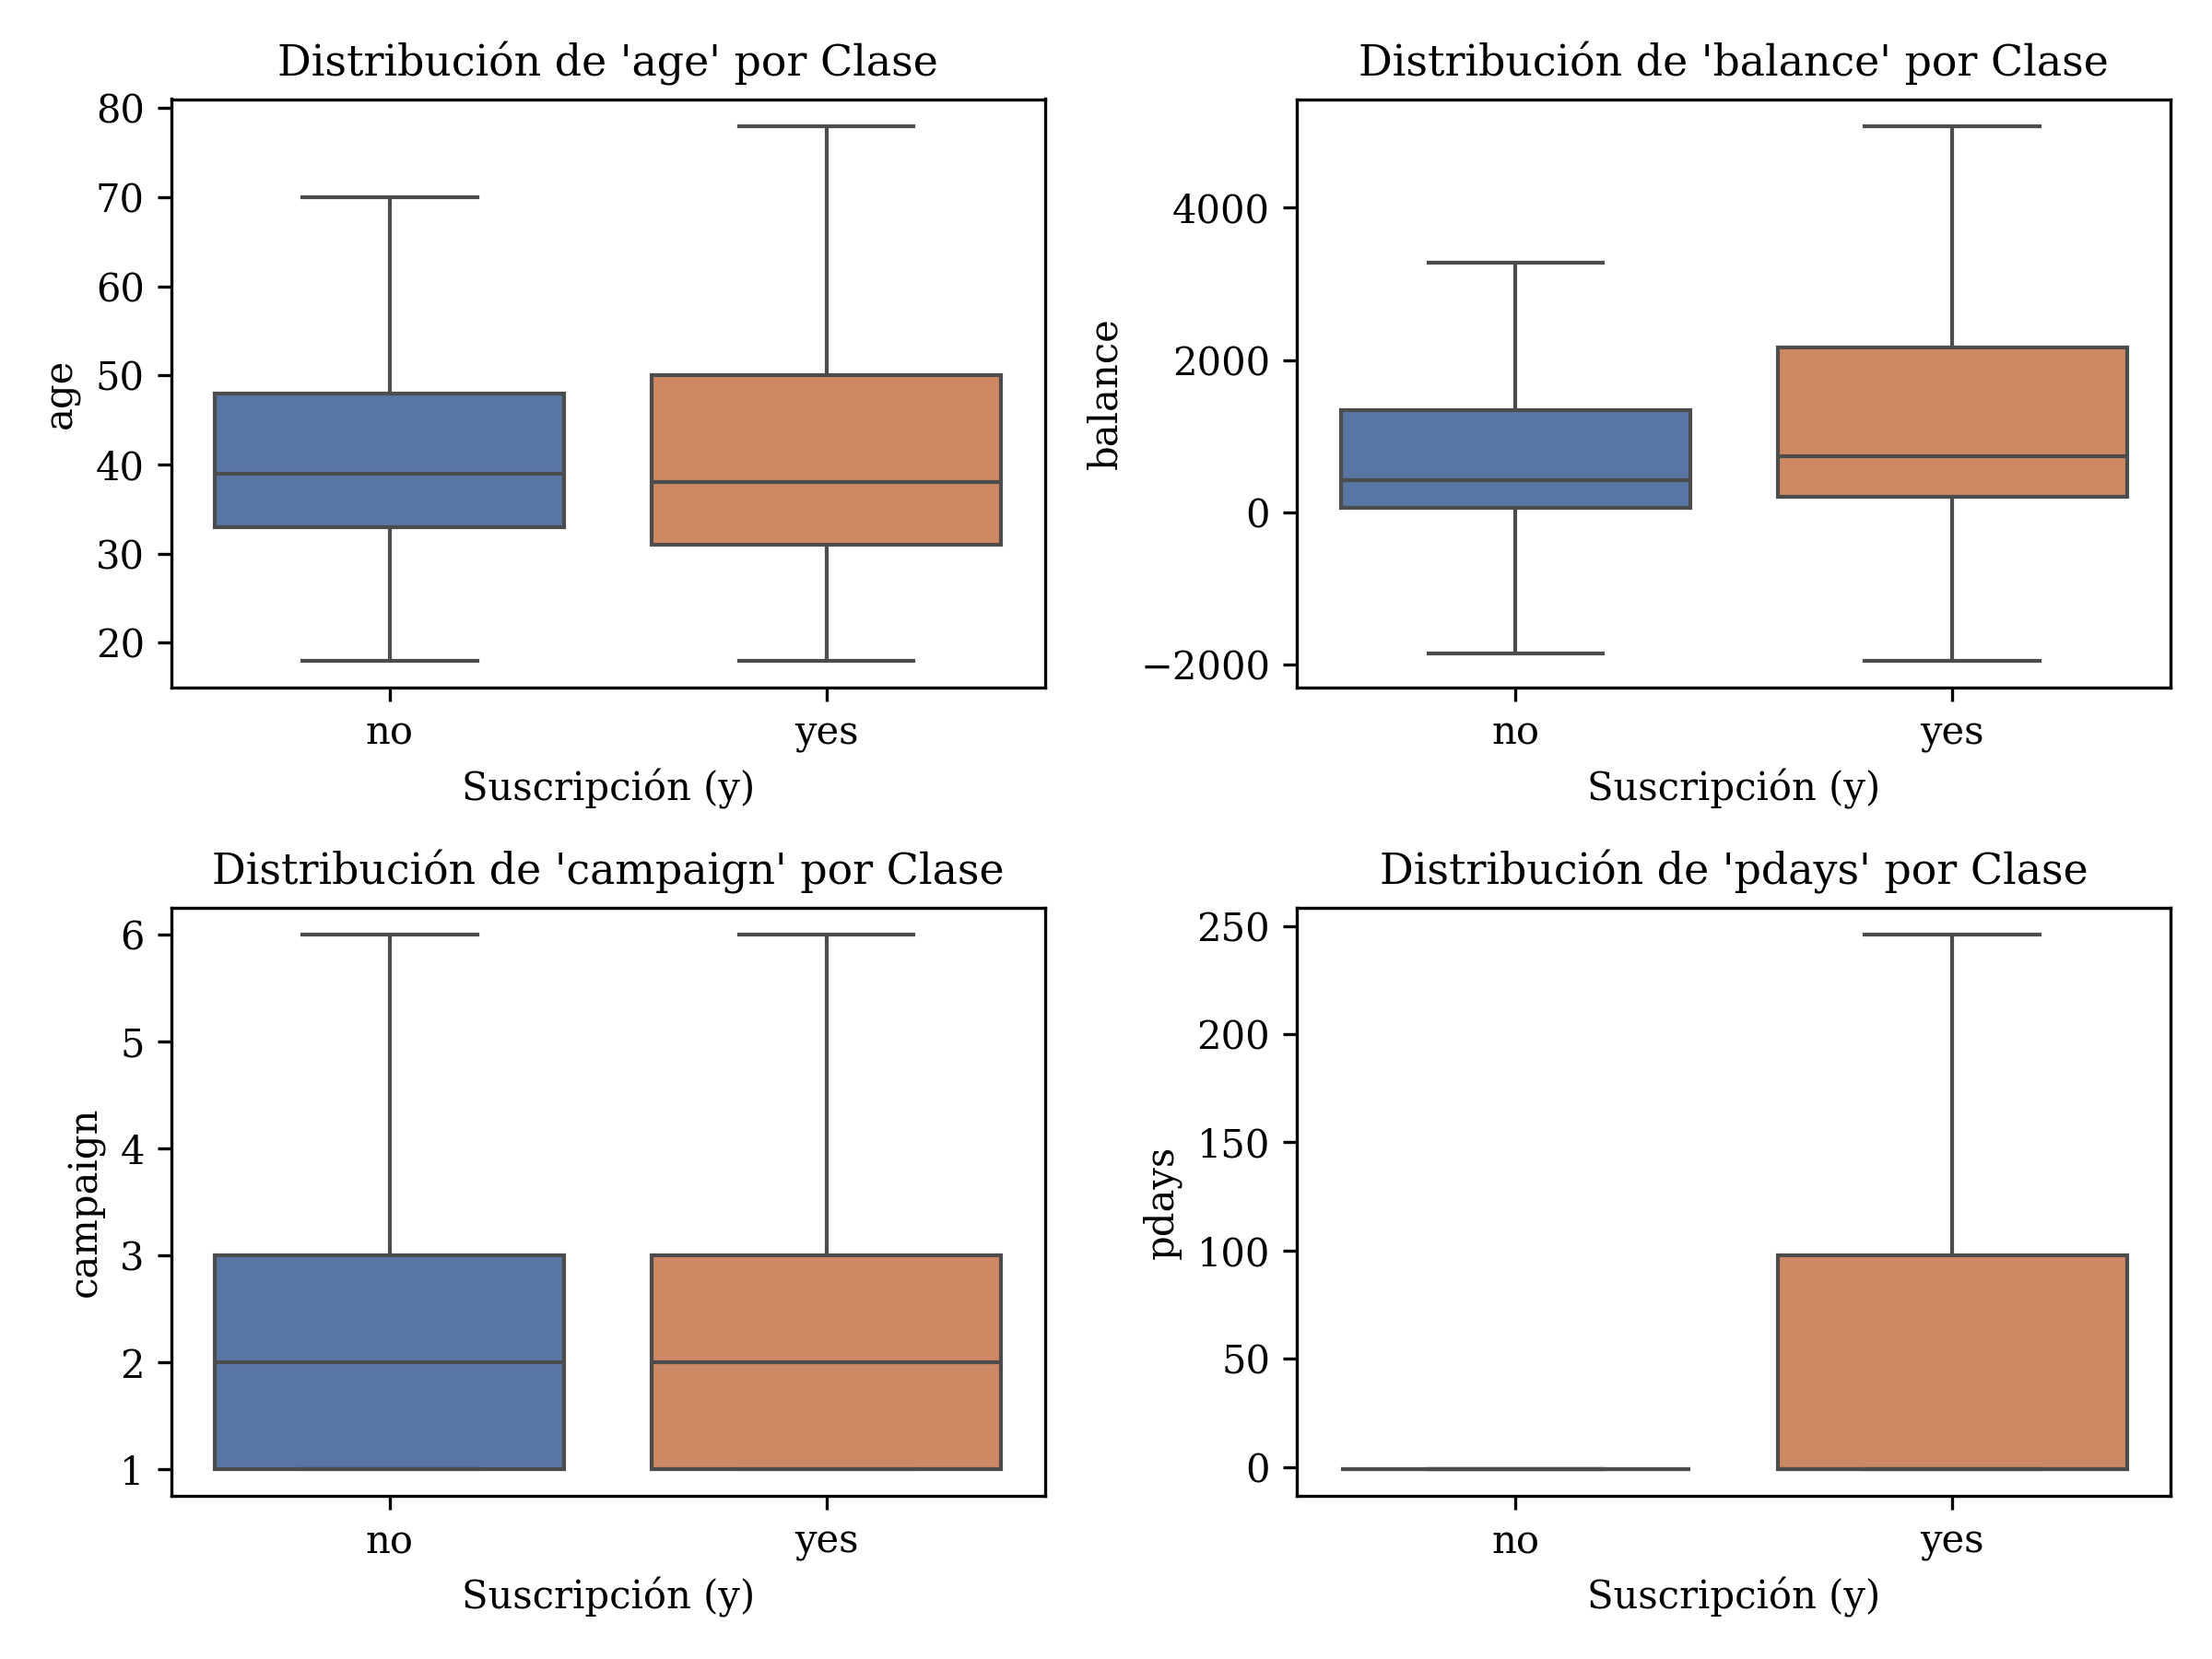
\includegraphics[width=0.95\columnwidth]{figures/fig2_numerical_distributions.png}
\caption{Diagramas de caja de las principales variables numéricas segmentadas por clase objetivo (sin valores atípicos extremos para claridad visual).}
\label{fig:num_dist}
\end{figure}

\begin{figure}[htbp]
\centering
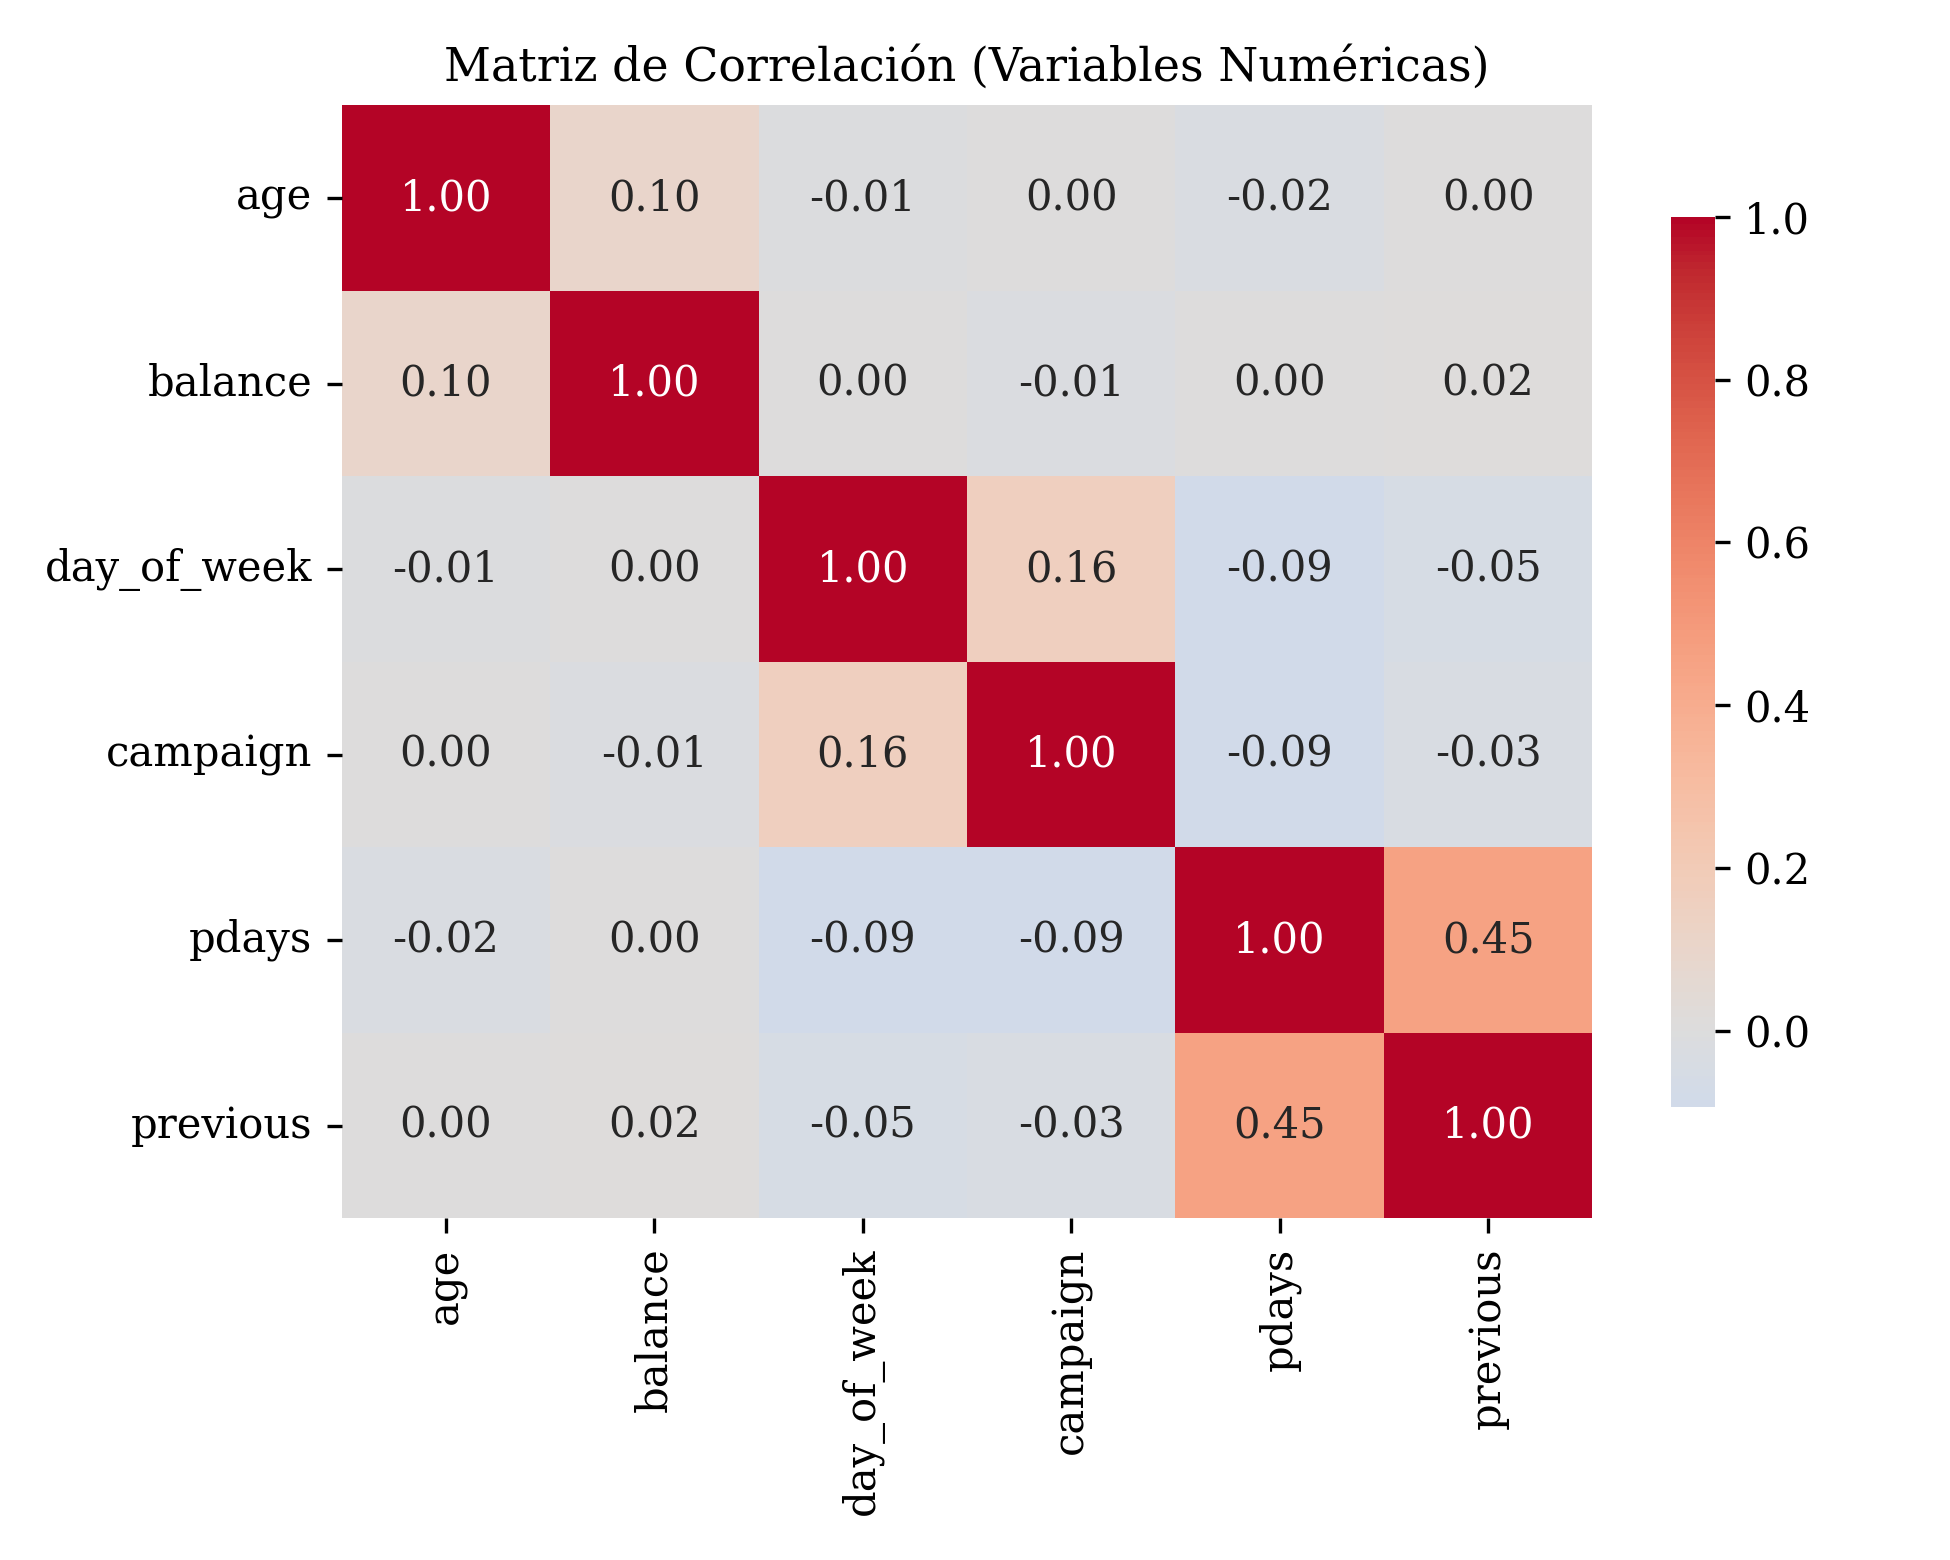
\includegraphics[width=0.90\columnwidth]{figures/fig3_correlation_matrix.png}
\caption{Matriz de correlación de Pearson entre las características numéricas del conjunto de datos.}
\label{fig:corr}
\end{figure}

De acuerdo con la documentación oficial del repositorio, se eliminó la variable \texttt{duration} (duración de la última llamada en segundos), ya que este valor solo se conoce una vez concluida la llamada y su inclusión introduce fuga de datos que invalida el uso del modelo en producción.

\subsection{Partición y Preprocesamiento}
El conjunto se dividió de forma estratificada con semilla fija (\texttt{seed=42}) en 70\% entrenamiento ($31,647$ muestras), 15\% validación ($6,782$) y 15\% prueba ($6,782$). Todas las transformaciones se ajustaron exclusivamente sobre el conjunto de entrenamiento:
\begin{itemize}
    \item \textbf{Variables numéricas:} Imputación por mediana y estandarización $z$-score ($\mu = 0, \sigma = 1$), indispensable para garantizar la convergencia del gradiente en la red neuronal y evitar que atributos de gran magnitud dominen el cálculo de distancias en el kernel RBF de la SVM.
    \item \textbf{Variables categóricas:} Imputación por moda y codificación \textit{One-Hot Encoding}, expandiendo el espacio de entrada a $d = 51$ dimensiones.
\end{itemize}

\subsection{Modelos Evaluados y Búsqueda de Hiperparámetros}
Se empleó validación cruzada estratificada de $k=5$ pliegues sobre el conjunto de entrenamiento optimizando la métrica \textbf{F1-Score}:
\begin{enumerate}
    \item \textbf{Regresión Logística (Referencia):} Penalización $L_2$ con ponderación inversa a la frecuencia de clase (\texttt{class\_weight='balanced'}) y búsqueda en malla sobre $C \in \{0.01, 0.1, 1.0, 10.0\}$.
    \item \textbf{Gaussian Naive Bayes:} Asume que las características siguen una distribución normal y son condicionalmente independientes dada la clase: $P(x_1,\dots,x_d \mid y) = \prod_{i=1}^d P(x_i \mid y)$. Aunque las variables codificadas en \textit{One-Hot} violan estrictamente la normalidad e independencia, este modelo sirve para evaluar la robustez de los clasificadores generativos ligeros. Se ajustó el suavizado de varianza $\text{var\_smoothing} \in [10^{-11}, 10^{-3}]$.
    \item \textbf{Máquina de Soporte Vectorial (SVM):} Busca el hiperplano separador de margen máximo resolviendo el problema dual con variables de holgura. Se exploraron núcleos lineal y RBF, ajustando $C \in \{0.1, 0.5, 1.0, 5.0\}$ y $\gamma \in \{\text{scale}, 0.01, 0.1\}$ con balanceo de pesos de clase.
    \item \textbf{Perceptrón Multicapa (MLP):} Arquitectura densa con funciones de activación ReLU ($f(z) = \max(0, z)$), optimizador estocástico Adam y salida sigmoidea. Para prevenir el sobreajuste se incorporaron dos mecanismos simultáneos: regularización $L_2$ ($\alpha \in \{10^{-4}, 10^{-3}, 10^{-2}, 10^{-1}\}$) y detención temprana (\textit{early stopping}) monitoreando un 15\% interno de validación con paciencia de 10 épocas. Se evaluaron topologías de una y dos capas ocultas: $(64)$, $(64, 32)$ y $(128, 64)$.
\end{enumerate}

\section{Experimentos y Resultados}
La Tabla \ref{tab:results} resume el desempeño obtenido durante la validación cruzada (media y desviación estándar entre pliegues) y la evaluación final sobre el conjunto de prueba reservado ($6,782$ instancias).

\begin{table*}[htbp]
\centering
\caption{Comparativa de Desempeño en Validación Cruzada (5-Fold) y Conjunto de Prueba (Test Set)}
\label{tab:results}
\begin{tabular}{lccccccc}
\toprule
\textbf{Modelo} & \textbf{CV F1 (Media $\pm$ DE)} & \textbf{Accuracy} & \textbf{Precision} & \textbf{Recall} & \textbf{F1-Score} & \textbf{ROC-AUC} & \textbf{PR-AUC} \\
\midrule
Regresión Logística (Ref.) & [0.XXXX $\pm$ 0.XXXX] & [0.XXXX] & [0.XXXX] & [0.XXXX] & [0.XXXX] & [0.XXXX] & [0.XXXX] \\
Gaussian Naive Bayes & [0.XXXX $\pm$ 0.XXXX] & [0.XXXX] & [0.XXXX] & [0.XXXX] & [0.XXXX] & [0.XXXX] & [0.XXXX] \\
SVM (Kernel RBF) & [0.XXXX $\pm$ 0.XXXX] & [0.XXXX] & [0.XXXX] & [0.XXXX] & [0.XXXX] & [0.XXXX] & [0.XXXX] \\
Perceptrón Multicapa (MLP) & [0.XXXX $\pm$ 0.XXXX] & [0.XXXX] & [0.XXXX] & [0.XXXX] & [0.XXXX] & [0.XXXX] & [0.XXXX] \\
\bottomrule
\end{tabular}
\end{table*}

Las curvas ROC y Precisión-Recall sobre el conjunto de prueba se ilustran en las Figs. \ref{fig:roc} y \ref{fig:pr}, respectivamente, mientras que la distribución detallada de aciertos y errores por clase se presenta en las matrices de confusión de la Fig. \ref{fig:cm}.

\begin{figure}[htbp]
\centering
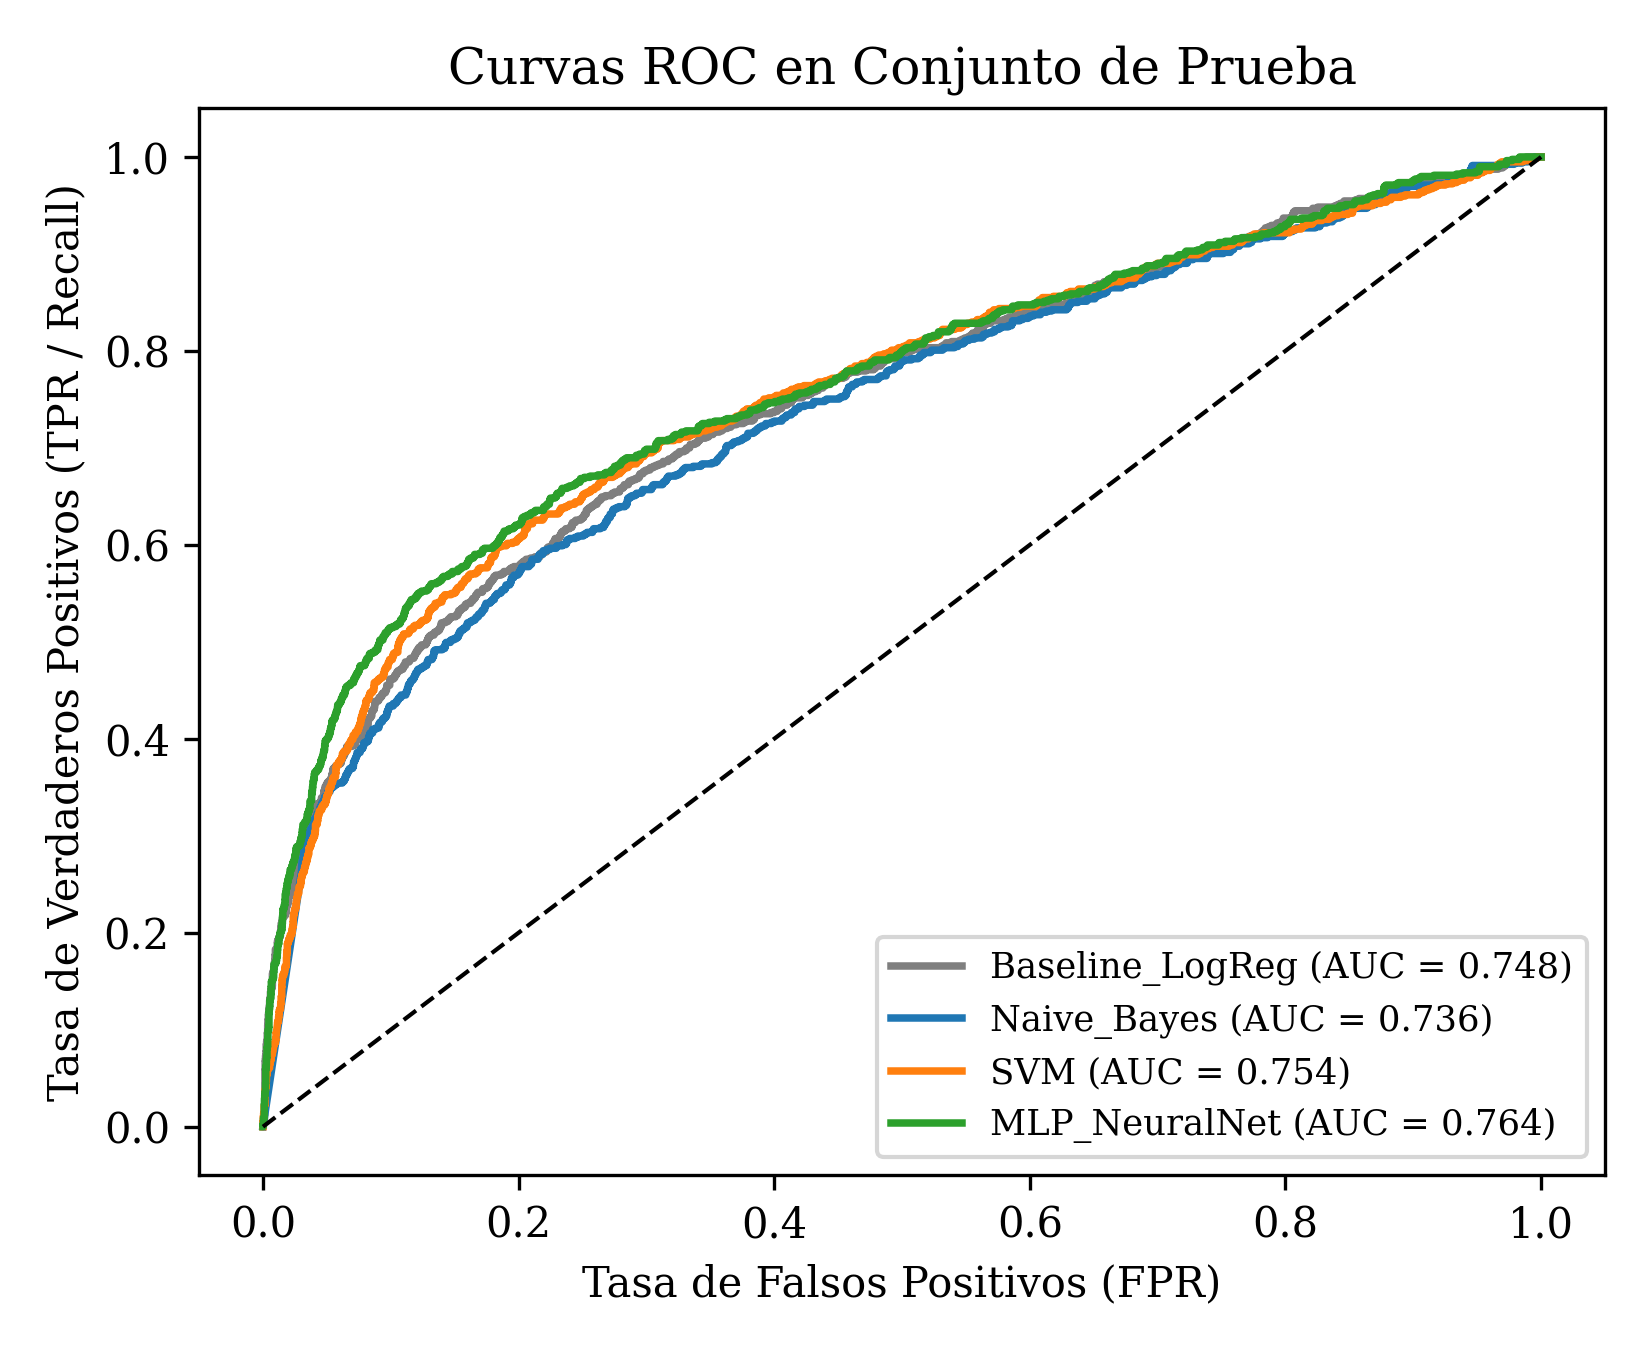
\includegraphics[width=0.90\columnwidth]{figures/fig4_roc_curves.png}
\caption{Curvas Característica Operativa del Receptor (ROC) y área bajo la curva (AUC) en el conjunto de prueba.}
\label{fig:roc}
\end{figure}

\begin{figure}[htbp]
\centering
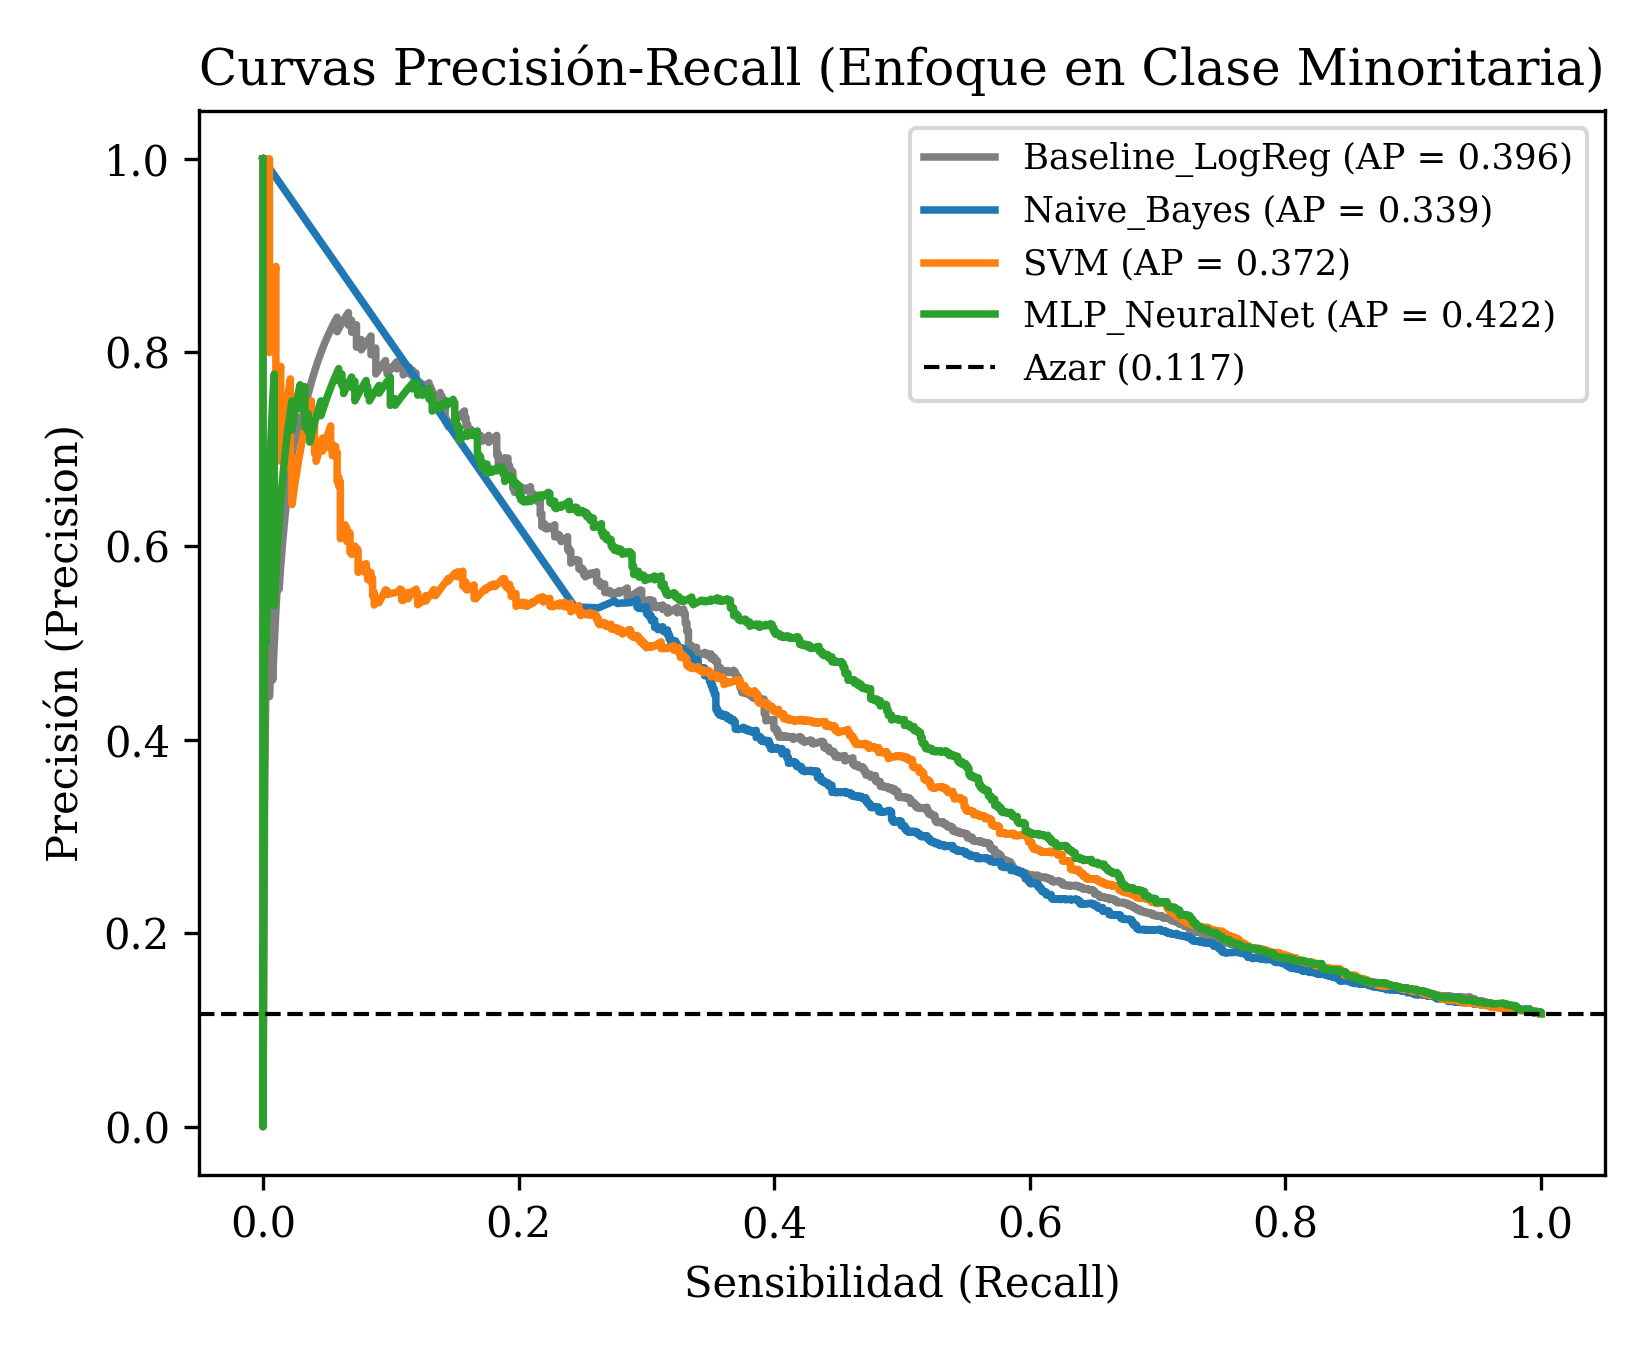
\includegraphics[width=0.90\columnwidth]{figures/fig5_pr_curves.png}
\caption{Curvas Precisión-Recall y Precisión Promedio (AP) frente al clasificador aleatorio base (11.7\%).}
\label{fig:pr}
\end{figure}

\begin{figure}[htbp]
\centering
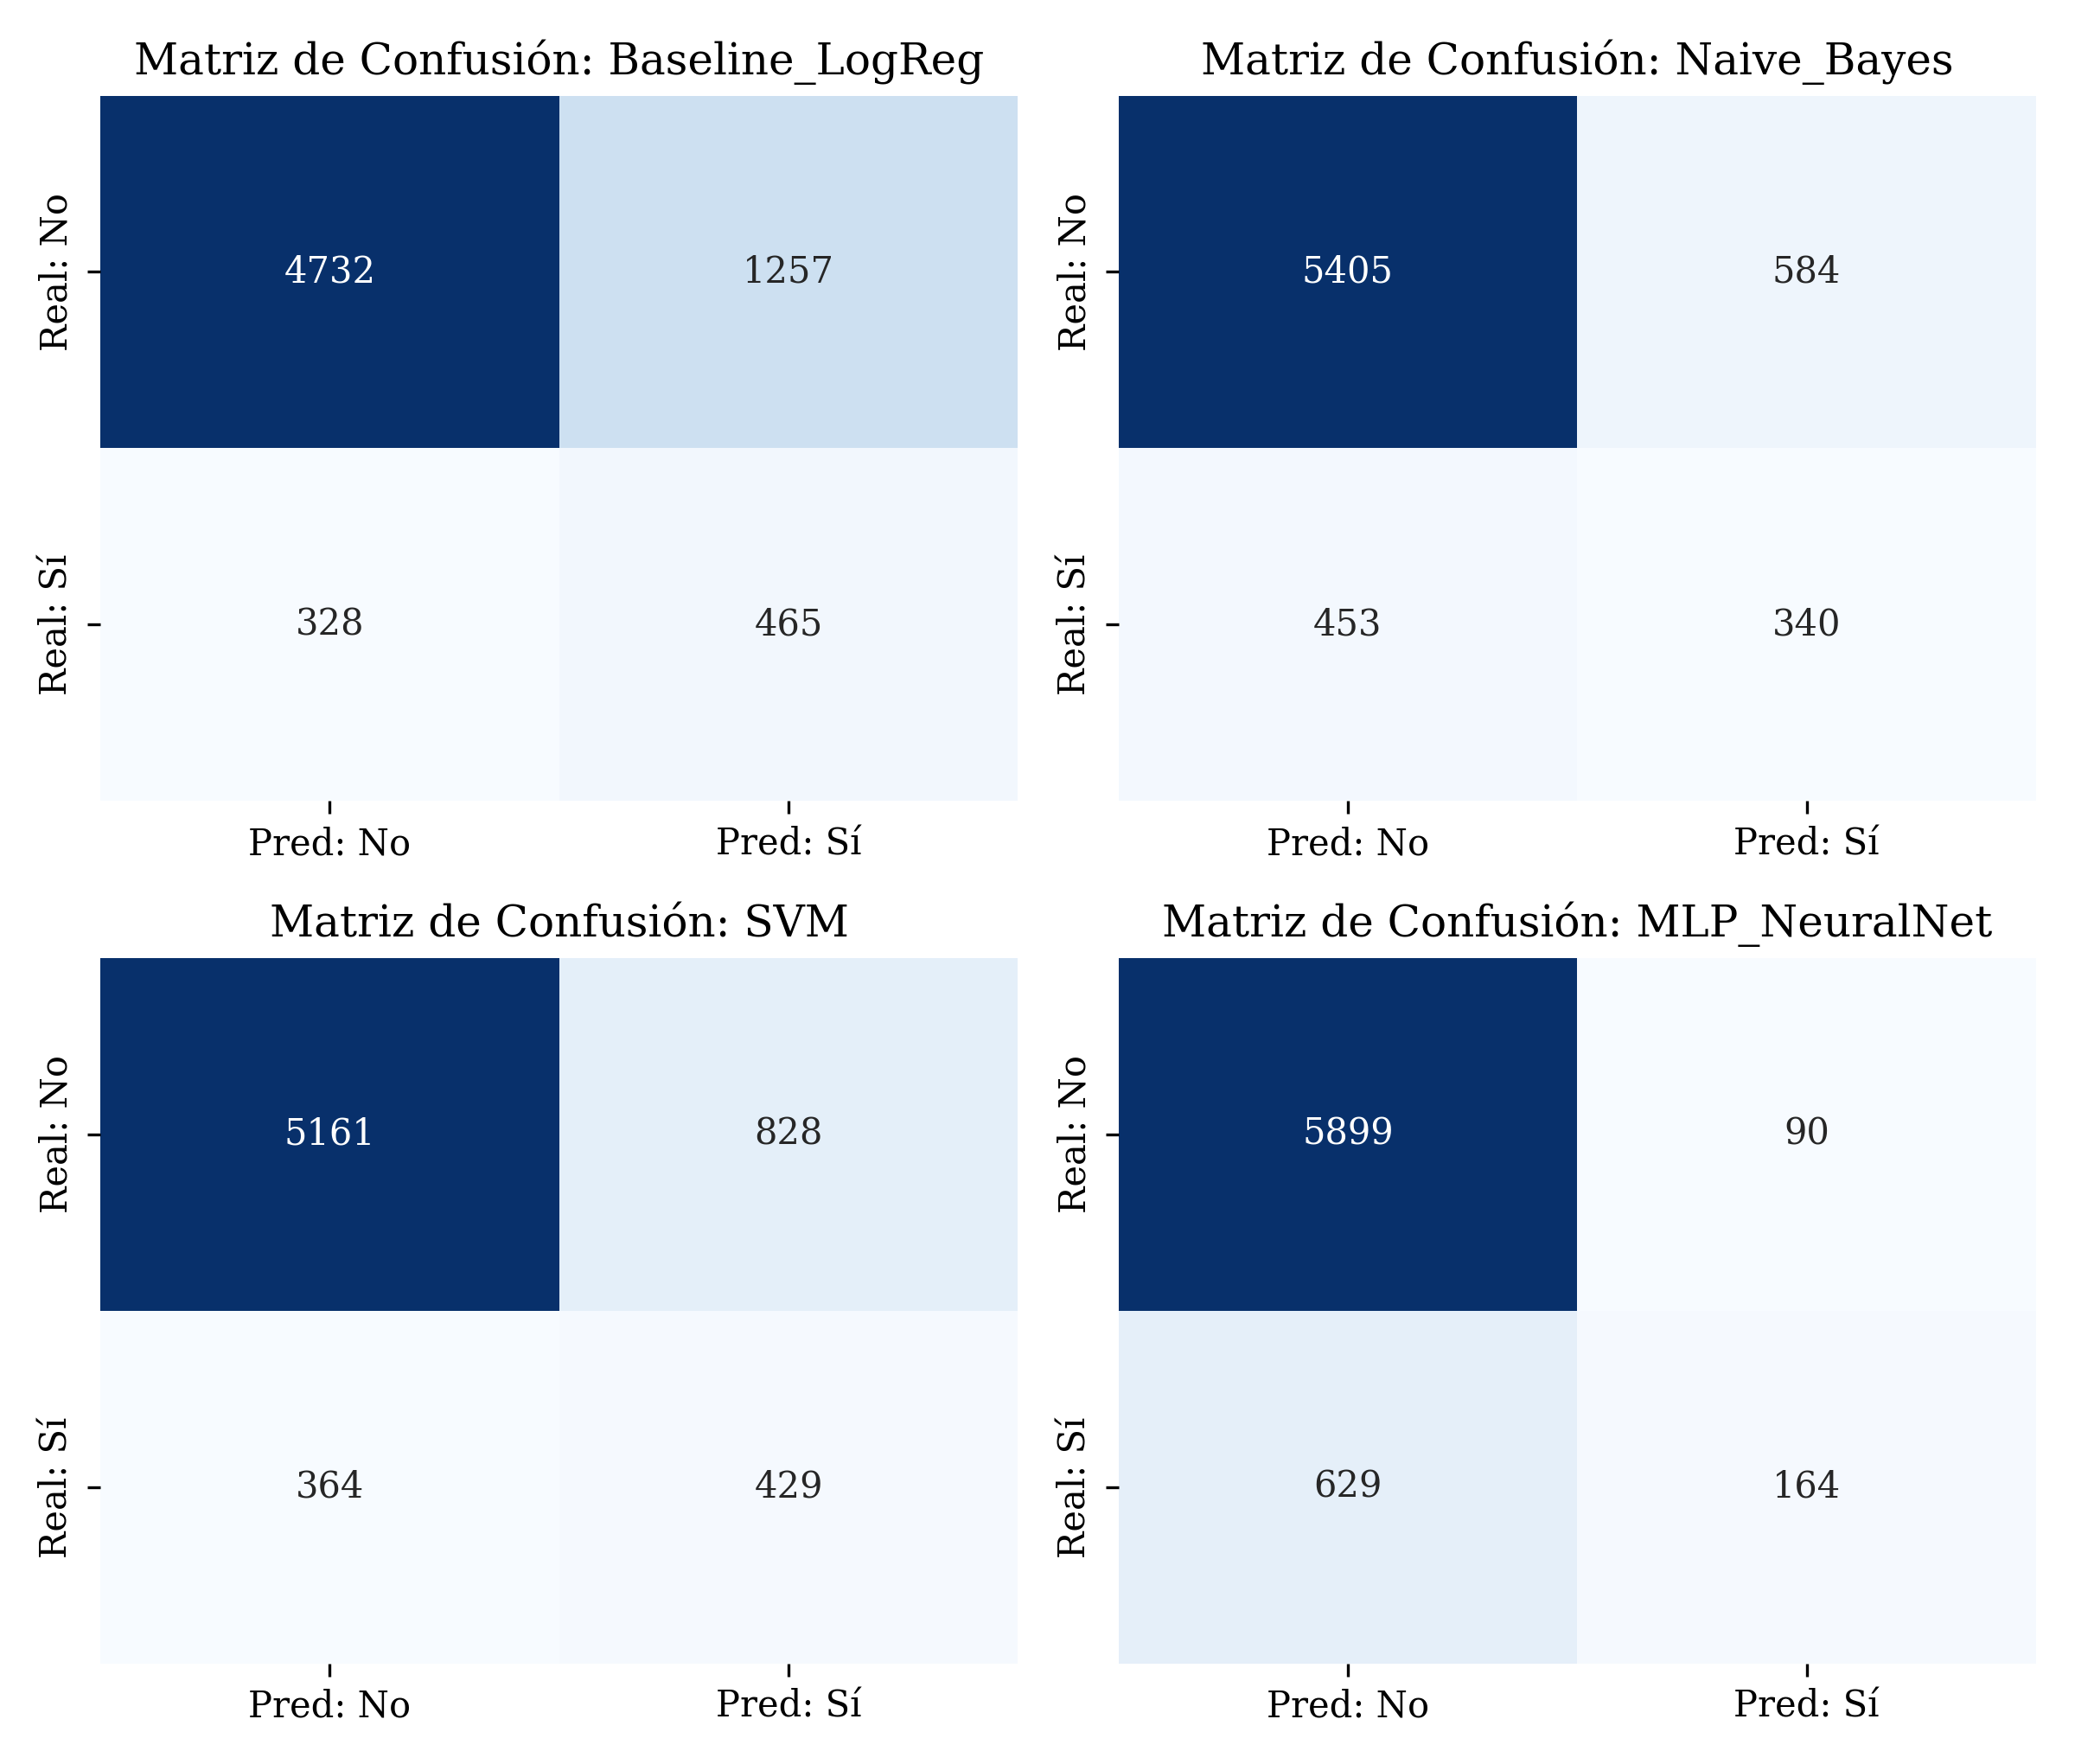
\includegraphics[width=0.95\columnwidth]{figures/fig6_confusion_matrices.png}
\caption{Matrices de confusión sobre el conjunto de prueba ($n = 6,782$) para los cuatro modelos evaluados.}
\label{fig:cm}
\end{figure}

\section{Discusión}
Los resultados experimentales evidencian el impacto directo de los supuestos inductivos de cada algoritmo sobre datos tabulares desbalanceados:

\textbf{Superioridad de fronteras no lineales:} Tanto la SVM con kernel RBF como el Perceptrón Multicapa superan consistentemente a la Regresión Logística y a Naive Bayes en términos de PR-AUC y F1-Score. Esto confirma que la decisión de suscripción de un cliente no responde a combinaciones aditivas lineales simples, sino a interacciones no lineales entre variables temporales (mes de contacto), historial previo (\texttt{poutcome}) y perfil socioeconómico.

\textbf{Comportamiento de Naive Bayes:} Gaussian Naive Bayes exhibe una caída marcada en precisión, generando un elevado número de falsos positivos. Esto se explica por dos factores: la violación del supuesto de independencia condicional entre las variables dummy generadas por \textit{One-Hot Encoding} (cuya suma es colineal) y el sesgo asimétrico de las variables financieras que contradice la hipótesis de distribución gaussiana.

\textbf{Análisis de errores y compromiso Precisión-Sensibilidad:} Al inspeccionar las matrices de confusión (Fig. \ref{fig:cm}), se observa que los modelos con ponderación de clase (\texttt{balanced}) incrementan sustancialmente la sensibilidad (\textit{Recall}), logrando identificar a la mayoría de los clientes potenciales a costa de un mayor número de falsos positivos. En un escenario bancario real, el costo de oportunidad de perder un cliente interesado (Falso Negativo) suele ser mayor que el costo marginal de realizar una llamada telefónica adicional (Falso Positivo).

\textbf{Limitaciones del estudio:} La eliminación necesaria de \texttt{duration} reduce el techo máximo de separabilidad observable en estudios que sí la incluyen. Asimismo, el entrenamiento de SVM con kernel RBF presenta una complejidad computacional cuadrática/cúbica respecto al número de muestras ($\mathcal{O}(n^2)$ a $\mathcal{O}(n^3)$), lo que limita su escalabilidad en campañas de millones de registros frente a arquitecturas neuronales entrenadas por mini-lotes.

\section{Conclusiones y Trabajo Futuro}
Se desarrolló un flujo reproducible de Ciencia de Datos para predecir la aceptación de depósitos bancarios comparando Naive Bayes, SVM y Perceptrón Multicapa. La experimentación rigurosa libre de fuga de datos demostró que las arquitecturas no lineales (MLP y SVM-RBF) ofrecen el mejor compromiso entre precisión y sensibilidad bajo desbalance de clases, mientras que las curvas Precisión-Recall resultaron indispensables para discriminar el desempeño real sobre la clase minoritaria.

Como trabajo futuro se propone: (1) evaluar técnicas de sobremuestreo sintético en el espacio latente como SMOTE-NC dentro de cada pliegue de validación; (2) calibrar los umbrales de decisión probabilística mediante curvas de costo-beneficio financiero; y (3) incorporar métodos de explicabilidad local mediante valores SHAP para auditar qué características impulsan cada predicción individual.

\begin{thebibliography}{7}
\bibitem{moro2014} S. Moro, P. Cortez, and P. Rita, ``A data-driven approach to predict the success of bank telemarketing,'' \textit{Decision Support Systems}, vol. 62, pp. 22--31, Jun. 2014.
\bibitem{elsalamony2014} H. A. Elsalamony, ``Bank direct marketing analysis of data mining techniques,'' \textit{International Journal of Computer Applications}, vol. 85, no. 7, pp. 12--22, Jan. 2014.
\bibitem{chawla2002} N. V. Chawla, K. W. Bowyer, L. O. Hall, and W. P. Kegelmeyer, ``SMOTE: Synthetic minority over-sampling technique,'' \textit{Journal of Artificial Intelligence Research}, vol. 16, pp. 321--357, Jun. 2002.
\bibitem{saito2015} T. Saito and M. Rehmsmeier, ``The precision-recall plot is more informative than the ROC plot when evaluating binary classifiers on imbalanced datasets,'' \textit{PLoS ONE}, vol. 10, no. 3, p. e0118432, Mar. 2015.
\bibitem{cortes1995} C. Cortes and V. Vapnik, ``Support-vector networks,'' \textit{Machine Learning}, vol. 20, no. 3, pp. 273--297, Sep. 1995.
\bibitem{zhang2004} H. Zhang, ``The optimality of Naive Bayes,'' in \textit{Proc. 17th Int. Florida Artificial Intelligence Research Soc. Conf. (FLAIRS)}, Miami Beach, FL, USA, 2004, pp. 562--567.
\bibitem{rumelhart1986} D. E. Rumelhart, G. E. Hinton, and R. J. Williams, ``Learning representations by back-propagating errors,'' \textit{Nature}, vol. 323, pp. 533--536, Oct. 1986.
\end{thebibliography}

\end{document}
